\subsection{Product Functions}
%%%%%
%All the system features, i.e. all the functional requirements for the application
%%%%%


\normalsize
\vspace{12pt}


\subsubsection{Set Password : FRQ1}
\textbf{(Source: Bernard Wagner, Priority: Medium)}
\begin{itemize}
\item A user must be able to set a password for local authentication purposes.
\end{itemize}
%------------------------------------------------------------------------------------------------------------
\subsubsection{Edit Password : FRQ2}
\textbf{(Source: Group Deliberation, Priority: Medium)}
\begin{itemize}
\item The user must be able to edit the authenticating password.
\end{itemize}
%------------------------------------------------------------------------------------------------------------
\subsubsection{Local Authentication : FRQ3}%meaning functional requirement 3
\textbf{(Source: Bernard Wagner, Priority: Medium)}
\begin{itemize}
\item The application must authenticate a user by requiring a password in order to log into the application, in order to ensure confidentiality.
\end{itemize}
%------------------------------------------------------------------------------------------------------------
\subsubsection{Enter message : FRQ4}%meaning functional requirement 1
\textbf{(Source: Bernard Wagner, Priority: High)}
\begin{itemize}
\item A user must be able to input text into the application.
\end{itemize}
%------------------------------------------------------------------------------------------------------------
\subsubsection{Type message : FRQ4.1}
\textbf{(Source: Bernard Wagner, Priority: High)}
\begin{itemize}
\item A user must be able to type text into the application.
\end{itemize}
%------------------------------------------------------------------------------------------------------------
\subsubsection{Paste message : FRQ4.2}
\textbf{(Source: Bernard Wagner, Priority: High)}
\begin{itemize}
\item A user must be able to paste an already conducted message into the application, using the clipboard.
\end{itemize}
%------------------------------------------------------------------------------------------------------------
\subsubsection{Edit Message: FRQ5}
\textbf{(Source: Bernard Wagner, Priority: Medium)}
\begin{itemize}
\item The message text must be editable once it has been input into the application by the user.
\end{itemize}
%------------------------------------------------------------------------------------------------------------
\subsubsection{Encrypt message : FRQ6}
\textbf{(Source: Bernard Wagner, Priority: High)}
\begin{itemize}
\item The message must be encrypted using a suitable encryption method.
\end{itemize}
%------------------------------------------------------------------------------------------------------------
\subsubsection{Copy Encrypted Message : FRQ7}
\textbf{(Source: Bernard Wagner, Priority: High)}
\begin{itemize}
\item Once a message has been encrypted, a user must be able to copy the ciphertext, and paste it into a suitable messaging application.
\end{itemize}
%------------------------------------------------------------------------------------------------------------
\subsubsection{Decrypt message : FRQ8}
\textbf{(Source: Bernard Wagner, Priority: High)}
\begin{itemize}
\item The application must be able to decrypt the message (on the receiving end) to reveal the original text.
\end{itemize}
%------------------------------------------------------------------------------------------------------------
\subsubsection{Add Contact : FRQ9}
\textbf{(Source: Bernard Wagner, Priority: High)}
\begin{itemize}
\item Before communicating with someone, the receiver must be added as a contact, in order to be able to communicate with that user.
\end{itemize}
%------------------------------------------------------------------------------------------------------------
\subsubsection{Edit Contact : FRQ10}
\textbf{(Source: Bernard Wagner, Priority: Medium)}
\begin{itemize}
\item A contact must be editable once it has been added.
\end{itemize}
%------------------------------------------------------------------------------------------------------------
\subsubsection{Remove Contact : FRQ11}
\textbf{(Source: Bernard Wagner, Priority: High)}
\begin{itemize}
\item A user must be able to remove a contact.
\end{itemize}
%------------------------------------------------------------------------------------------------------------


\subsection{i* Diagrams}
\subsubsection{General i* diagram}
SMSEncryption General i* diagram

\begin{center}
 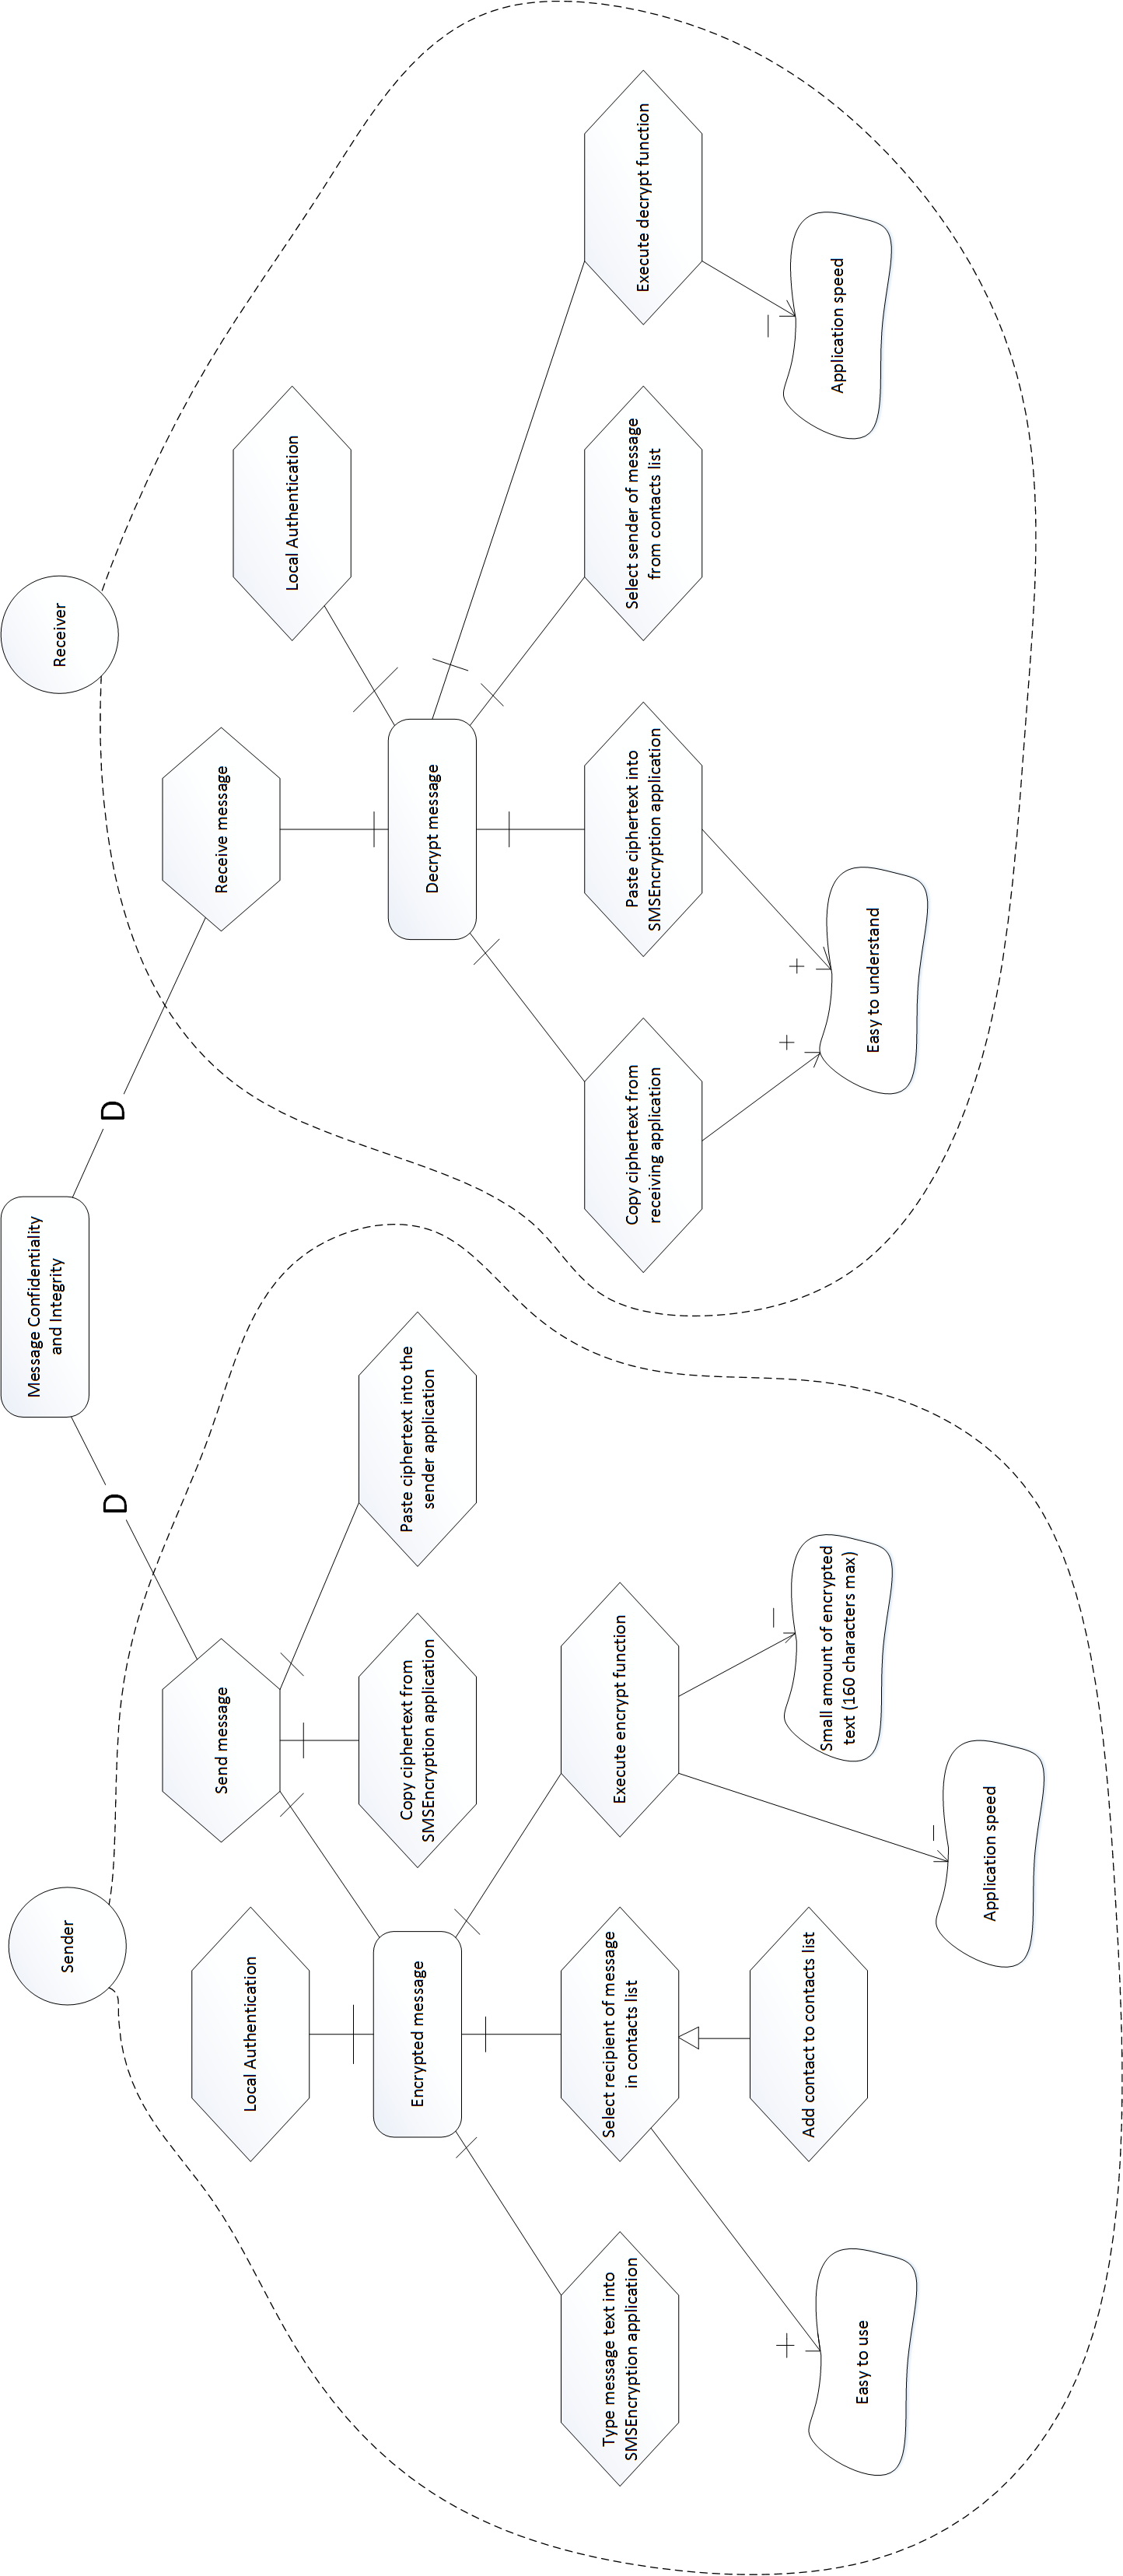
\includegraphics[width=13cm]{diagrams/IStarDiagrams/SMSEncryptionIStarDiagram.png}
\end{center}
